\documentclass[11pt]{beamer}
\title{Probabilistic Program Analysis with Martingales}
\usepackage{verbatim}
\usepackage{amsmath}
\usepackage{amsthm}
\usepackage{listings}
\usepackage{graphics}
\usepackage{color}
\usepackage{multicol}
\usepackage{stmaryrd}\usefonttheme[onlymath]{serif}

\newtheorem{proposition}{Proposition}
\author{Aleksandar Chakarov and Sriram Sankaranarayanan\\
CAV'13
}
\date{Report date: \today}





\begin{document}
\maketitle
\begin{frame}\frametitle{Introduction}

\begin{itemize}
\item 
Probablistic programs: Standard imperative program + \emph{random value generators}


\begin{itemize}
\item Branching.

\item Assignment.

\end{itemize}

\item 
Problem: Invariant synthesis and termination checking in probablistic settings.



\end{itemize}
\end{frame}

\begin{frame}\frametitle{Contributions}
\begin{itemize}
\item Extend \emph{quantitative invariants} using Azuma-Hoeffding theorem to generate probabilistic assertions.

\item Define \emph{super martigale ranking functions} (SMRF) to prove almost sure termination ($\texttt{Pr}(terminates) = 1$) of probablistic programs.
\item A constraint-based algorithm for supermartingale expression generation.
\end{itemize}
\end{frame}

\begin{frame}\frametitle{Restrictions}

\begin{itemize}

\item Only applies to stochastic programs. (Not a demonic program with non-determinism)

\item Restricted on linear expressions and systems.

\item A.s. termination proving is sound but incomplete.
\end{itemize}
\end{frame}

\begin{frame}\frametitle{Motivating Examples}
\begin{example}

\begin{center}
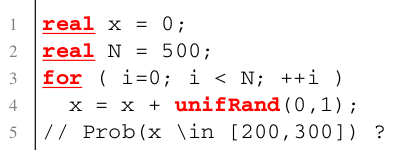
\includegraphics[scale=0.4]{1.png}
\end{center}

\begin{itemize}
\item Traditional invariant at loop exit: $0\le x \le 501 \wedge i = N$

\item Probablistic assertion: $ \texttt{Pr}(x\in [200, 300]) \ge  0.84$
\end{itemize}

\end{example}
\end{frame}

\begin{frame}\frametitle{Motivating Examples}
\begin{example}[Hare and Tortoise]
\begin{center}
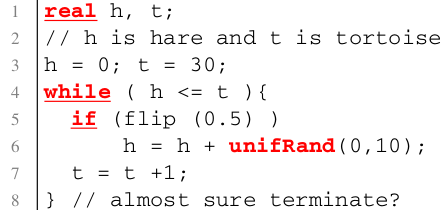
\includegraphics[scale=0.4]{2.png}
\end{center}
\begin{itemize}
\item Worst case: non-terminating.
\item The expression $t - h$ decrease by $1.5$ in expectation each iteration.
\end{itemize}
\end{example}


\end{frame}


\begin{frame}\frametitle{Probablistic Transition System}
\begin{center}
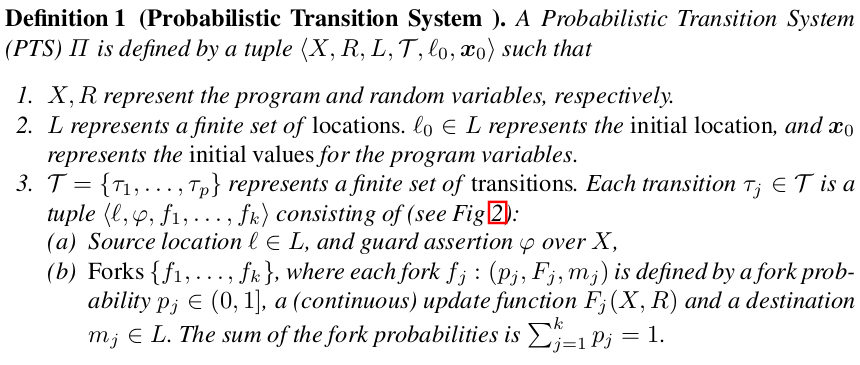
\includegraphics[scale=0.35]{def1.png}

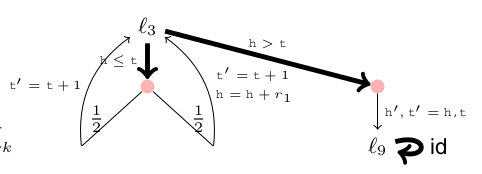
\includegraphics[scale=0.35]{def1exp.png}
\end{center}

\textbf{No Demonic:} mutually exclusive and mutually exhaustive.
\end{frame}

\begin{frame}\frametitle{State and Post-Distribution}

A \emph{state} of PTS is a tuple $(l,\mathbf{x})$ where $
l\in L$ and $\mathbf{x}$ is a valuation of $X$.

Given a transition $\tau = \langle l, \phi, f_1, \ldots, f_k\rangle $, if $\mathbf{x}\models \phi$ then the result of executing $\tau$ is a \emph{probability distribution} over post states, obtained by:

\begin{enumerate}
\item Choose fork $f_j$ with probability $p_j$, and a vector of random variables $\mathbf{r}:(r_1, \ldots, r_m)$ is drawn according to the joint distribution.


\item Update the states by computing the function $\mathbf{x}' = F_j(\mathbf{x}, \mathbf{r})$ and update $l$ to $m_j$. 
\end{enumerate}

\[
\textsc{Post-Distrib}(s,\tau), \textsc{Post-Distrib}(s)\]

Operationally, PTS is a Markov chain.
\end{frame}

\begin{frame}\frametitle{State and Post-Distribution}

\begin{center}
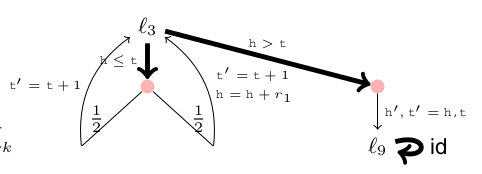
\includegraphics[scale=0.4]{def1exp.png}
\end{center}

\end{frame}

\begin{frame}\frametitle{Sampled Executions}
\begin{center}
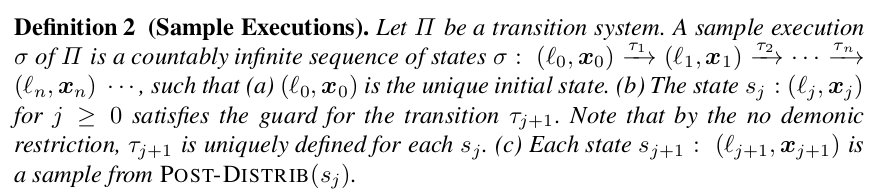
\includegraphics[scale=0.35]{def2.png}
\end{center}
\begin{example}

\begin{center}
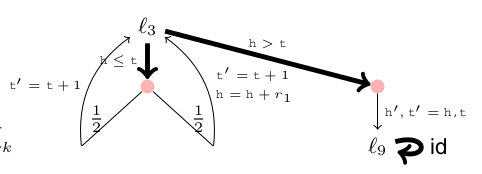
\includegraphics[scale=0.3]{def1exp.png}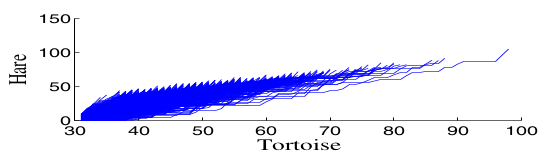
\includegraphics[scale=0.3]{def2exp.png}
\end{center}

\end{example}




\end{frame}


\begin{frame}\frametitle{Almost Sure Termination}

\begin{definition}[Termination]

Let $\Pi$ be a PTS with a special \emph{final location} $l_F$. $l_F$ has only one outgoing transition $\texttt{id}$. A sampled execution $\sigma$ of $\Pi$ \emph{terminates} if it eventually reaches a state $(l_F, \mathbf{x})$ .

\end{definition}

Probability of terminating paths:

\begin{itemize}
\item For a finite syntactic path $\pi:l_0\stackrel{\tau_1}{\rightarrow} l_1 \stackrel{\tau_2}{\rightarrow}l_2\ldots l_F$, there is a well-defined probaility $\mu(\pi)\in[0,1]$ that characterizes the probaility of the path going through the locations.

\item The overall probability of termination can be obtained as the sum of probability of all such finite syntactic paths.
\end{itemize}


\end{frame}


\begin{frame}\frametitle{Almost Sure Termination}

The main idea to show $\mu$ on the infinite space is well-defined:

Let $\Omega = \Pi_{j = 1}^\infty \Omega_j$ and $\mathcal{F} = \Pi_{j = 1}^\infty \mathcal{F}_j$.

\begin{itemize}
\item 
At each location $l_i$, there is a probability  space $(\Omega_i, \mathcal{F}_i, \mu_i)$. 
\item 
For a given $n$, a measurable cylinder can be constructed by $B_n = \{\omega\in \Omega \mid (\omega_1, \ldots, \omega_n)\in B^n\}$, where $B^n = \Pi^n_{j = 1}A_j, A_j\in \mathcal{F}_j$. Assume the measure is $P_n$.
\item Theorem of cylinder construction, a probability measure space $(\Omega, \mathcal{F}, P)$ such that $P\{\omega\in\Omega\mid (\omega_1, \ldots, \omega_n)\in B^n\} = P_n(B^n)$.
\end{itemize}



\end{frame}

\begin{frame}\frametitle{Almost Sure Termination}
\begin{definition}[a.s. Termination]
A PTS is said to be almost sure terminating iff the sum of probabilities of all  terminating syntactic paths is $1$.
\end{definition}
\end{frame}
\begin{frame}\frametitle{Pre-Expectation}
\begin{definition}[Pre-expectation of an expression]
Let state $s:(l,\mathbf{x})$ be a state and $\tau$ be the enabled transition on $s$. The pre-expectation $\mathbb{E}(\mathbf{e}'|s)$ is defined as the conditional expected value of $\mathbf{e}'$ over $\mathtt{Post-Distrib}(s)$ as 
\[\mathbb{E}_\tau(\mathbf{e}'|s) = \Sigma_{j = 1}^k p_j\mathbb{E}_R(\mathtt{pre}(\mathbf{e}', F_j))\]
\end{definition}
\end{frame}

\begin{frame}\frametitle{Pre-Expectation}
\begin{center}
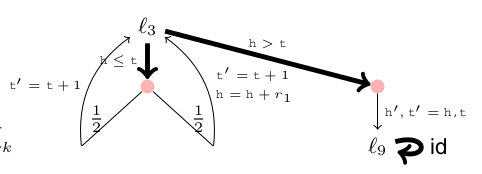
\includegraphics[scale=0.4]{def1exp.png}
\end{center}
\begin{example}
\[\mathbb{E}(5t-2h|(l_3, h, t))\]

\end{example}

\end{frame}

\begin{frame}\frametitle{Martingale and Supermartingale Expression}
\begin{center}
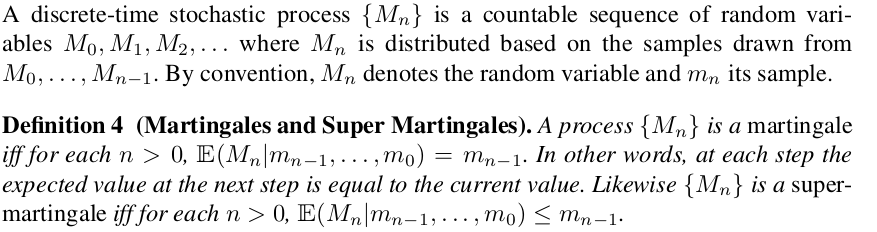
\includegraphics[scale=0.35]{def:martingale.png}
\end{center}
Adapting the original definition to PTS:
\begin{center}
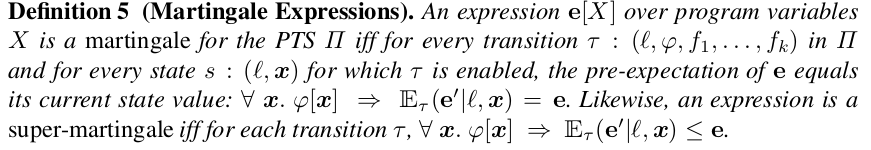
\includegraphics[scale=0.35]{def:martingaleexp.png}
\end{center}
\end{frame}

\begin{frame}\frametitle{From Martingale to Probabilistic Assertion}

\begin{center}
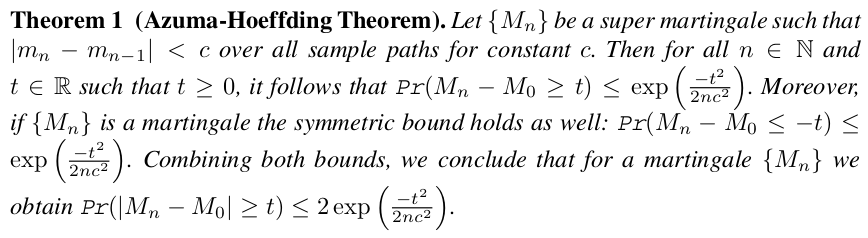
\includegraphics[scale=0.35]{azuma.png}
\end{center}

\end{frame}

\begin{frame}\frametitle{Almost-Sure Termination}

\begin{definition}[Ranking Super Martingale(RSM)]

A supermartingale $\{M_n\}$ is ranking iff
\begin{itemize}
\item There exists $\epsilon > 0$ s.t. for all sampled paths, $\mathbb{E}(M_{n+1}|m_n) \le m_n - \epsilon$.

\item For all $n\ge 0$, $M_n \ge -K$ for some $K >0$. 

(Equiv. Def. For all $n\ge 0$, $M_n\ge 0$).
\end{itemize}
\end{definition}
\end{frame}

\begin{frame}\frametitle{How a.s. Termination is Proved?}
Ranking function: will finally become negative.

Ranking Supermartingale: will almost surely be come negative.
\pause
\begin{theorem}[Main result]
A ranking supermartingale with a positive initial value will a.s. become negative.
\end{theorem}
\pause
\begin{proof}
Stopping time: $t = \inf_{n\ge 0} m_n\le 0$. Let the r.v. be $T$.
$M_{n}^{T}$. 
$Y_n = M_{n}^{T} + \epsilon\min(n,T)$.
\end{proof}
\pause
\begin{lemma}
$\{Y_n\}$ is a super martingale and $Y_n \ge -K$
\end{lemma}

\end{frame}


\begin{frame}\frametitle{How to Synthesize SMRF}

\end{frame}

\end{document}